\documentclass{standalone}
\usepackage{tikz}
\makeatletter\AtBeginDocument{\@buildstepset{0,1,2}}\makeatother
\usetikzlibrary{intersections, calc}
\usepackage{hsbcommon}
    \begin{document}
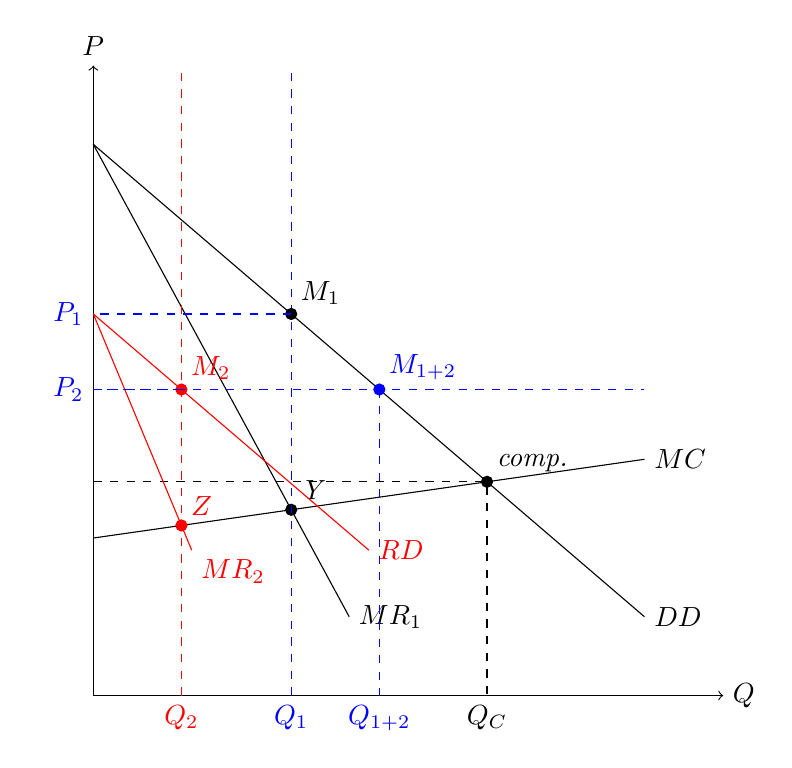
\begin{tikzpicture}[remember picture]
        \draw[->] (0,0) node[below] {\phantom{$X_i$}} -- (8,0) node[right] (Q) {$Q$};
        \draw[->] (0,0) node[left] {\phantom{$Y_mi$}} -- (0,8) node[above] (P) {$P$};

        \coordinate (A) at (0,7);
        \coordinate (F) at ($(A) +(7,-6)$);
        % \coordinate (F) at (7,1);
 
        \draw [name path=demand] {(A) -- (F)};
        \node[right] at (F) {$DD$};

        % Demand curve

        \coordinate (G) at (0,2);
        \coordinate (L) at (7,3);
        
        \draw [name path=supply]  {(G) -- (L)};
        \node[right] at (L) {$MC$};

        %% COMPETITION CASE
            
            \path [name intersections={of=demand and supply,by=X}];
    
            \filldraw (X) circle (2pt) node[above right] {\textit{comp.}};
            \draw[dashed] (0,|-X) -- (X) -- (X|-,0) node[below] {$Q_C$};
    
            % \draw[dashed, red] (0,0) rectangle (X);
            
            % \draw [dashed,red ] (X |-, 0) node[below] {$Q_C$}-- (X |-, 8);
            % \draw[red, dashed] (X) -- (0, |- X) node[left] {$P_C$};

        %% MONOPOLY CASE
        
            % \coordinate (M) at (0,8);
            % \coordinate (B) at (2,6);
            % \coordinate (C) at (3,4);
            % \coordinate (D) at (4,3);
            % \coordinate (E) at (6,2);

            %% draw profit parablola
            % \coordinate (M) at (0,3) ;
            % \coordinate (N) at (2.5,8);
            % \coordinate (O) at (5,3);
            % \draw[dashed] (M) plot [smooth,tension=1] coordinates {(M) (N) (O)};
            
            \coordinate (N) at (3.25,1);
     
            \draw [name path=mr] plot [smooth] coordinates {(A) (N)};
            \node[right] at (N) {$MR_1$};
    
            \path [name intersections={of=mr and supply,by=Y}];
            \filldraw (Y) circle (2pt) node[above right] {\textit{Y}};
    
            \draw [name path=mono, dashed,blue ] (Y |-, 0) node[below] {$Q_1$} -- (Y |-, 8);
            \path [name intersections={of=mono and demand,by=Z}];
            
            \filldraw (Z) circle (2pt) node[above right] {\textit{$M_1$}};
            \draw[blue, dashed] (Z) -- (0, |- Z) node[left] {$P_1$};
    
        %% residual Demand

        \ifstep{1}{
            \begin{scope}[color=red]

            \coordinate (B) at (0,|- Z);
            \coordinate (E) at ($(B) + (3.5,-3)$);
            % \coordinate (E) at (5,1);
            \draw [name path=resdemand] plot [smooth] coordinates {(B) (E)};
            \node[right] at (E) {$RD$};        
    
            \coordinate (G) at ($(B) + (1.25,-3)$);;
            % \coordinate (G) at (2.5,1);
     
            \draw [name path=mrzwei] plot [smooth] coordinates {(B) (G)};
            \node[below right] at (G) {$MR_2$};
    
            \path [name intersections={of=mrzwei and supply,by=Z}];
            \filldraw (Z) circle (2pt) node[above right] {$Z$};

            \draw [name path=monozwei, dashed] (Z |-, 0) node[below] {$Q_2$} -- (Z |-, 8);
            \path [name intersections={of=monozwei and resdemand,by=Q}];
            
            \filldraw (Q) circle (2pt) node[above right] {\textit{$M_2$}};
 
        \end{scope}
    }
    \ifstep{2}{
        \begin{scope}[blue]
            
            \draw[dashed] (Q) -- (0, |- Q) node[left] {$P_2$};

            \draw[name path=pm2,dashed] (0, |- Q) -- (7, |- Q);
            \path[name intersections={of=pm2 and demand,by=R}];
            \filldraw (R) node[above right] {$M_{1+2}$} circle (2pt);
            \draw[dashed] (R) -- (R |-,0) node[below] {$Q_{1+2}$};
        \end{scope}
    }       

        
    \end{tikzpicture}
\end{document}
